\documentclass{beamer}
\usetheme{metropolis} % Clean modern look

\usepackage{amsmath, amsfonts}
\usepackage{graphicx}
\usepackage{booktabs}
\usepackage{hyperref}

\title{Performance Analysis in Machine Learning}
\subtitle{}
\date{}

\begin{document}

% Title Slide
{
\setbeamertemplate{frame footer}{\href{https://github.com/abkafi1234/Datamining_MachineLearning_Class/tree/main/Class_Slides}{Report Error}}
\setbeamerfont{frame footer}{size=\tiny} 
\begin{frame}
    \titlepage
\end{frame}
}

% Outline Slide
\begin{frame}{Outline}
    \tableofcontents
\end{frame}


% Overview
\section{Overview of Key Metrics}
\begin{frame}{Overview of Key Metrics}
\begin{itemize}
  \item MSE: Mean Squared Error
  \item RMSE: Root Mean Squared Error
  \item R²: Coefficient of Determination
  \item ROC-AUC: Area Under the ROC Curve
  \item Confusion Matrix
  \item Precision
  \item Recall
  \item F1 Score
\end{itemize}
\end{frame}

% Section: MSE
\section{MSE (Mean Squared Error)}

\begin{frame}{MSE: Definition and Formula}
\textbf{Definition:} Average of squared prediction errors.

\[
\text{MSE} = \frac{1}{n} \sum_{i=1}^{n} (y_i - \hat{y}_i)^2
\]

\begin{itemize}
  \item Lower is better.
  \item Sensitive to large errors.
\end{itemize}
\end{frame}

\begin{frame}{MSE: Example}
\textbf{Actual values:} \( y = [3, -0.5, 2, 7] \)

\textbf{Predicted values:} \( \hat{y} = [2.5, 0.0, 2, 8] \)

\vspace{0.3cm}
\[
\text{MSE} = \frac{1}{4}[(3 - 2.5)^2 + (-0.5 - 0.0)^2 + (2 - 2)^2 + (7 - 8)^2]
\]
\[
= \frac{1}{4}[0.25 + 0.25 + 0 + 1] = \frac{1.5}{4} = 0.375
\]
\end{frame}

% Section: RMSE
\section{RMSE (Root Mean Squared Error)}

\begin{frame}{RMSE: Formula and Intuition}
\[
\text{RMSE} = \sqrt{\frac{1}{n} \sum_{i=1}^{n}(y_i - \hat{y}_i)^2}
\]

\begin{itemize}
  \item Same units as the target variable.
  \item Interpretable and commonly reported.
\end{itemize}
\end{frame}

\begin{frame}{RMSE: Example}
Using the same MSE as before:

\[
\text{MSE} = 0.375 \quad \Rightarrow \quad \text{RMSE} = \sqrt{0.375} \approx 0.612
\]
\end{frame}

% Section: R²
\section{R² (Coefficient of Determination)}

\begin{frame}{R²: Formula and Meaning}
\[
R^2 = 1 - \frac{\sum (y_i - \hat{y}_i)^2}{\sum (y_i - \bar{y})^2}
\]

\begin{itemize}
  \item Measures proportion of variance explained.
  \item \( R^2 = 1 \): perfect model
  \item \( R^2 = 0 \): same as predicting mean
\end{itemize}
\end{frame}

\begin{frame}{R²: Example}
\textbf{Actual:} \( y = [1, 2, 3] \quad \hat{y} = [1.1, 1.9, 3.2] \)

\vspace{0.3cm}
Step 1: Mean \( \bar{y} = 2 \)

\vspace{0.3cm}
\[
\text{SS}_{\text{res}} = (1-1.1)^2 + (2-1.9)^2 + (3-3.2)^2 = 0.01 + 0.01 + 0.04 = 0.06
\]
\[
\text{SS}_{\text{tot}} = (1-2)^2 + (2-2)^2 + (3-2)^2 = 1 + 0 + 1 = 2
\]
\[
R^2 = 1 - \frac{0.06}{2} = 0.97
\]
\end{frame}



% <----------------------------->

\begin{frame}{Confusion Matrix: Definition}
A confusion matrix summarizes prediction results for binary classification:

\[
\begin{bmatrix}
\text{TP} & \text{FN} \\
\text{FP} & \text{TN} \\
\end{bmatrix}
\]

\begin{itemize}
  \item TP: True Positives
  \item TN: True Negatives
  \item FP: False Positives
  \item FN: False Negatives
\end{itemize}
\end{frame}

% Confusion Matrix - Dataset
\begin{frame}{Example Dataset}
\begin{tabular}{|c|c|c|}
\hline
\textbf{Email} & \textbf{Actual (Spam?)} & \textbf{Predicted (Spam?)} \\
\hline
1 & 1 & 1 \\
2 & 0 & 0 \\
3 & 1 & 1 \\
4 & 1 & 0 \\
5 & 0 & 1 \\
6 & 1 & 1 \\
7 & 0 & 0 \\
8 & 0 & 0 \\
9 & 1 & 0 \\
10 & 0 & 0 \\
\hline
\end{tabular}

\vspace{0.3cm}
From this we get:
\[
TP = 3,\quad FN = 2,\quad FP = 1,\quad TN = 4
\]
\end{frame}

% Precision
\begin{frame}{Precision}
\textbf{Definition:} Precision measures the proportion of predicted positives that are actually positive.

\[
\text{Precision} = \frac{TP}{TP + FP}
\]

\[
\text{Precision} = \frac{3}{3 + 1} = \frac{3}{4} = 0.75
\]

\textbf{Interpretation:} When the model predicts spam, it's correct 75\% of the time.
\end{frame}

% Recall
\begin{frame}{Recall}
\textbf{Definition:} Recall measures the proportion of actual positives that were correctly predicted.

\[
\text{Recall} = \frac{TP}{TP + FN}
\]

\[
\text{Recall} = \frac{3}{3 + 2} = \frac{3}{5} = 0.60
\]

\textbf{Interpretation:} The model catches 60\% of actual spam emails.
\end{frame}

% F1 Score
\begin{frame}{F1 Score}
\textbf{Definition:} Harmonic mean of precision and recall.

\[
F_1 = 2 \cdot \frac{\text{Precision} \cdot \text{Recall}}{\text{Precision} + \text{Recall}}
\]

\[
F_1 = 2 \cdot \frac{0.75 \cdot 0.60}{0.75 + 0.60} = \frac{0.90}{1.35} \approx 0.667
\]

\textbf{Interpretation:} Balanced measure that considers both false positives and false negatives.
\end{frame}

% Summary Table
\begin{frame}{Summary of Metrics}
\begin{tabular}{ll}
\toprule
\textbf{Metric} & \textbf{Value} \\
\midrule
True Positives (TP) & 3 \\
True Negatives (TN) & 4 \\
False Positives (FP) & 1 \\
False Negatives (FN) & 2 \\
\midrule
Precision & 0.75 \\
Recall & 0.60 \\
F1 Score & 0.667 \\
\bottomrule
\end{tabular}
\end{frame}

% <----------------------------->

% Section: ROC-AUC
\section{ROC-AUC (Classification)}

\begin{frame}{ROC-AUC: Concept}
\begin{itemize}
  \item ROC Curve: TPR(True Positive Rate) vs. FPR (False Positive Rate) at different thresholds.
  \item AUC: Area under the ROC curve.
  \item Measures the model’s ability to separate classes.
\end{itemize}

\text{AUC} = \text{Probability(model ranks a random positive} \\
\text{higher than a random negative)}
\end{frame}

\begin{frame}{ROC-AUC: Mini Example}
\textbf{True labels:} \( y = [0, 0, 1, 1] \)

\textbf{Predicted probs:} \( \hat{p} = [0.1, 0.4, 0.35, 0.8] \)\\
Threshold = 0.5
\begin{itemize}
  \item Pairwise comparisons of (positive, negative) → 4 pairs
  \item Model correctly ranks 3/4 → AUC = 0.75
\end{itemize}
\end{frame}


% Summary
\section{Summary}

\begin{frame}{Metric Comparison Summary}
\begin{itemize}
  \item \textbf{MSE, RMSE}: Use for regression error.
  \item \textbf{R²}: Goodness of fit in regression.
  \item \textbf{ROC-AUC}: Classifier performance independent of threshold.
  \item \textbf{Confusion Martix}: Confusion matrix provides the foundation for most classification metrics.
  \item \textbf{Precision}: Use Precision when false positives are costly.
  \item \textbf{Recall}: Use Recall when false negatives are costly.
  \item \textbf{F1Score}: F1 Score balances both — useful in imbalanced datasets.
\end{itemize}
\end{frame}

\section{More Important Metrics}
\begin{frame}{What Are Overfitting and Underfitting?}
  \begin{itemize}
    \item Two common modeling errors in machine learning.
    \item \textbf{Overfitting}: Model learns training data (and noise) too well.
    \item \textbf{Underfitting}: Model is too simple to capture patterns.
  \end{itemize}
  \vspace{0.5em}
  \textbf{Goal:} Build models that generalize well to unseen data.
\end{frame}

% Slide: Intuition
\begin{frame}{Intuition}
  \small
  \begin{itemize}
    \item \textbf{Overfit} → low bias, high variance
    \item \textbf{Underfit} → high bias, low variance
    \item We aim for the balance between bias and variance.
  \end{itemize}
  \vspace{1em}
  \begin{center}
    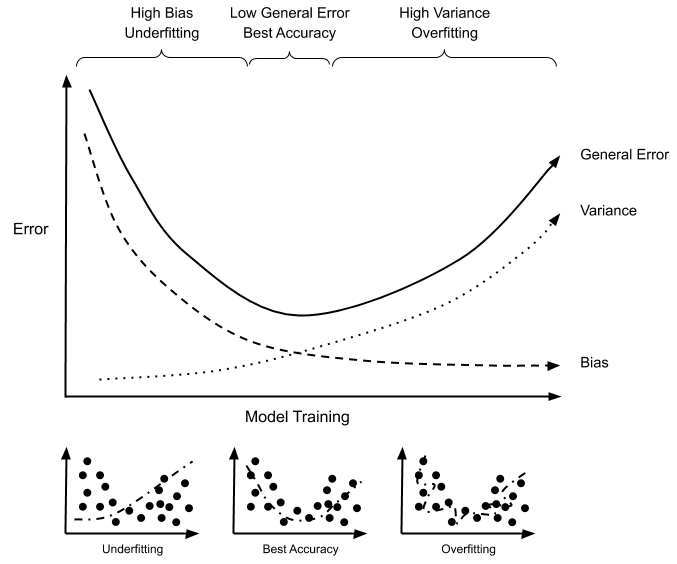
\includegraphics[width=0.6\textwidth]{Bias-Variance+Tradeoff.png}
  \end{center}
\end{frame}

% Slide: Overfitting
\begin{frame}{Overfitting}
  \textbf{Symptoms:}
  \begin{itemize}
    \item High training accuracy, low test accuracy
    \item Model too complex for the data
  \end{itemize}
  \vspace{0.5em}
  \textbf{Causes:}
  \begin{itemize}
    \item Too many features or parameters
    \item Training too long
    \item Small training set
  \end{itemize}
\end{frame}

% Slide: Fixing Overfitting
\begin{frame}{Fixing Overfitting}
  \textbf{Common solutions:}
  \begin{itemize}
    \item Use regularization (L1, L2)
    \item Early stopping
    \item Cross-validation
    \item Reduce model complexity
    \item Data augmentation
  \end{itemize}
\end{frame}

% Slide: Underfitting
\begin{frame}{Underfitting}
  \textbf{Symptoms:}
  \begin{itemize}
    \item Poor performance on both training and test sets
    \item Model fails to capture structure
  \end{itemize}
  \vspace{0.5em}
  \textbf{Causes:}
  \begin{itemize}
    \item Model too simple
    \item Insufficient training
    \item Too much regularization
  \end{itemize}
\end{frame}

% Slide: Fixing Underfitting
\begin{frame}{Fixing Underfitting}
  \textbf{Common solutions:}
  \begin{itemize}
    \item Increase model complexity
    \item Train longer (more epochs)
    \item Reduce regularization
    \item Improve features or transformations
  \end{itemize}
\end{frame}

% Slide: Visual Example
\begin{frame}{Visual Example}
  \begin{center}
    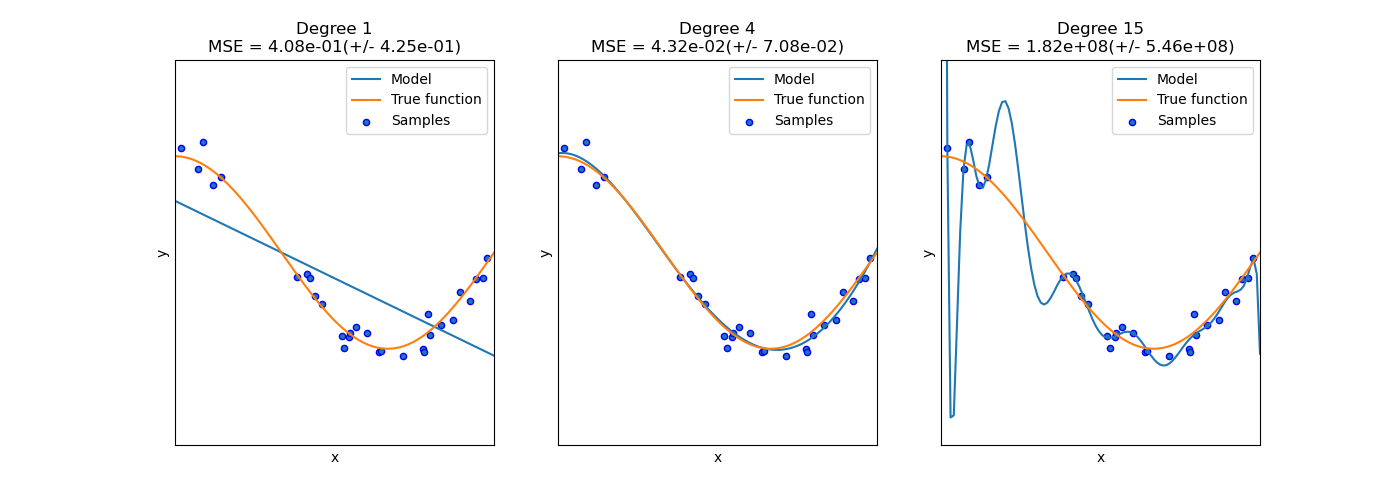
\includegraphics[width=0.9\textwidth]{sphx_glr_plot_underfitting_overfitting_001.png}
  \end{center}
  \footnotesize Source: Scikit-learn Documentation
\end{frame}

% Slide: Bias-Variance Table
\begin{frame}{Bias-Variance Tradeoff}
  \begin{tabular}{@{}ll@{}}
    \toprule
    \textbf{Metric} & \textbf{Behavior} \\
    \midrule
    Bias     & High in underfitting \\
    Variance & High in overfitting \\
    Goal     & Low bias and low variance \\
    \bottomrule
  \end{tabular}
\end{frame}

% Slide: How to Detect
\begin{frame}{How to Detect Overfitting and Underfitting}
  \begin{itemize}
    \item Compare training vs. validation error
    \item Plot learning curves
    \item Use cross-validation
    \item Monitor metrics: accuracy, loss, F1, etc.
  \end{itemize}
\end{frame}

% Slide: Python Example
\begin{frame}[fragile]{Python Example: Overfitting}
  \small
\begin{verbatim}
from sklearn.pipeline import make_pipeline
from sklearn.linear_model import LinearRegression
from sklearn.preprocessing import PolynomialFeatures
from sklearn.metrics import mean_squared_error

# Overfitting with high-degree polynomial
model = make_pipeline(PolynomialFeatures(15), LinearRegression())
model.fit(X_train, y_train)

print("Train Error:", mean_squared_error(y_train, model.predict(X_train)))
print("Test Error:", mean_squared_error(y_test, model.predict(X_test)))
\end{verbatim}
\end{frame}

% Slide: Best Practices
\begin{frame}{Best Practices}
  \begin{itemize}
    \item Always evaluate on unseen data
    \item Use regularization wisely
    \item Visualize performance over time
    \item Prefer simpler models when possible (Occam's Razor)
  \end{itemize}
\end{frame}


\begin{frame}[standout]
    Thank you!
\end{frame}
\end{document}
